\documentclass{article}

\usepackage[english]{babel}
\usepackage[utf8]{inputenc}
\usepackage{amsmath,amssymb}
\usepackage{parskip}
\usepackage{graphicx}
\usepackage[ruled,vlined]{algorithm2e}

\newcommand{\var}{\texttt}
\newcommand{\proc}[2]{\textsl{#1}(#2)}
\newcommand{\prop}{\textit}

\newcommand*{\escape}[1]{\texttt{\textbackslash#1}}
% Margins
\usepackage[top=2.5cm, left=3cm, right=3cm, bottom=4.0cm]{geometry}
% Colour table cells
\usepackage[table]{xcolor}

\newcommand{\tablespace}{\\[1.25mm]}
\newcommand\Tstrut{\rule{0pt}{2.6ex}}         % = `top' strut
\newcommand\tstrut{\rule{0pt}{2.0ex}}         % = `top' strut
\newcommand\Bstrut{\rule[-0.9ex]{0pt}{0pt}}   % = `bottom' strut

%%%%%%%%%%%%%%%%%
%     Title     %
%%%%%%%%%%%%%%%%%
\title{Scientific Computing Using Python - Assignment}
\author{Shreyas Srinivasa \\ shsr@es.aau.dk}
\date{\today}

\begin{document}
\maketitle

\section{Implementation}
The implementation for the assignment is performed with $4$ methods as suggested in the tasks. Implementation with each method is described below:

\subsection{Naive Version}
%Naive version%
The naive version is implemented with $2$-D arrays and $3$ methods: \textit{linspace()}, \textit{mandel\_naive()} and \textit{mandel\_set\_naive()}.
\begin{itemize}
    \item \textit{linspace(start, stop, n)} is used for creation of array with the start, stop and n variables denoting the range and the size. As per the project specification document, the values for start and stop are initialized. The function returns an array. The function is called for determining the real and imaginary parts of the array elements.
    \item \textit{mandel\_naive(c, maxiter, threshold)} calculates the value of \textit{z} as per the iterations and checks for the value bound for the threshold specified. The function returns the value for the mandelbrot set.
    \item \textit{mandel\_set\_naive(xmin,xmax,ymin,ymax,width,height,maxiter, threshold)} computes the mandelbrot set by initializing the real and imaginary parts. The parameters \textit{width} and \textit{height} represent the $p_{r_e}$ and $p_{i_m}$, \textit{maxiter} denotes the maximum iterations \textit{I} and the threshold represents \textit{T} . The function returns a list with the mandelbrot set. 
\end{itemize}

 
\subsection{Numba Version}
%Numba version%
The Numba version is similar to the naive version with an exception of using Numba \textit{@jit} decorator on top of the \textit{mandel\_naive()} function. As we run the program with multiple methods in a sequential execution, a seperate method is created called \textit{mandel\_numba()} with the \textit{@jit} decorator.

\subsection{Numba-Vectorized Version}
%Numba vectorised%
The vectorized version adds the \textit{@vectorize} decorator to create numba \textit{ufuncs} for parallelization. In the vectorization version, the method that computes the values for the mandelbrot set are changed to optimize the computation. The optimization is done through factoring out the redundant calculations by passing the real and imaginary parts of the complex numbers directly to the mandel function and calculating their squares separately only once and avoiding the square root computation by equations $1$, $2$ and $3$ that denote the definition of the square of complex numbers, the absolute value, and the sum of two complex numbers.

\begin{equation}
    (a+bi)^2=(a+bi)(a+bi)=(a^2-b^2)+2abi
   \end{equation}
\begin{equation}
    \left |(a+bi) \right |= \sqrt{a^2+b^2}
\end{equation}
\begin{equation}
       (a+bi)+(c+di)=(a+c)+(b+d)i
\end{equation}

The script \textit{variant.py} calls for parallelization of the method \textit{mandel\_numba\_vect} that computes the values for the mandelbrot set. The default number of threads set by numba in NUMBA\_NUM\_THREADS is $8$. On running the script, the vectorized methods run with this default value. However, to compare the execution time with different threads, the script \textit{vectorized.py} is called with a shell script \textit{vectorished.sh}. The number of script can be set in the shell script.  On executing the shell script, the execution time for the computation of the \textit{mandelset} is shown on the console. 


\subsection{Multiprocessing Version}
%Multiprocessing%
The Multiprocessing version utilizes the multiprocessing library. The method uses lists and the computation is distributed. To minimize the communication overhead, each task returns a row. The number of CPUs for computation is set by \textit{mp.cpu\_count()} as per the system configuration. However, this can be changed by specifying the value. The multiprocessing version also performs a loop to incorporate as many processors specified. 


\section{Output}
The output of the program are generated and stored in the \textit{/Output/} folder. THe folder is automatically created on first run and sub-folders are created on subsequent runs. The sub-folders are named as per the timestamp. The output folders contain the plots that are generated for each method, a table summarizing the execution times of each method and the simulation data. 

\subsection{Plots}
The plots are generated under the output folder for each implementation method. A sample plot that is generated can be seen in Figure \ref{fig:plot} below. 

\begin{figure}[h!]
    \centering
    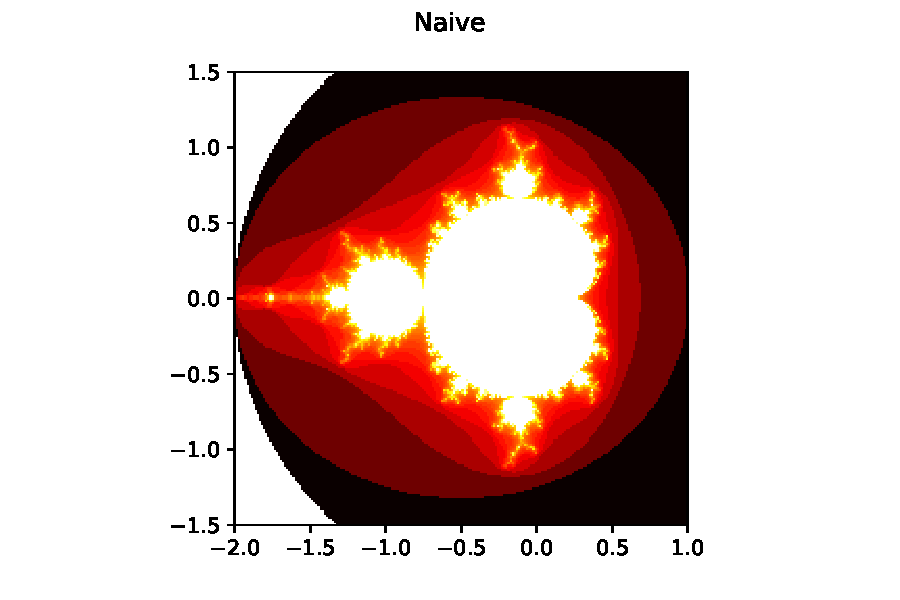
\includegraphics[scale=0.6]{Naive.pdf}
    \caption{Plot for the Naive Version}
    \label{fig:plot}
\end{figure}


\subsection{Execution Time}
The execution time for each implementation methods are summarized in the \textit{ExecutionTime.pdf} file. The file contains a table that shows the execution time for each method. An example of the file is seen in the Figure \ref{fig:exec} below.

\begin{figure}[h!]
    \centering
    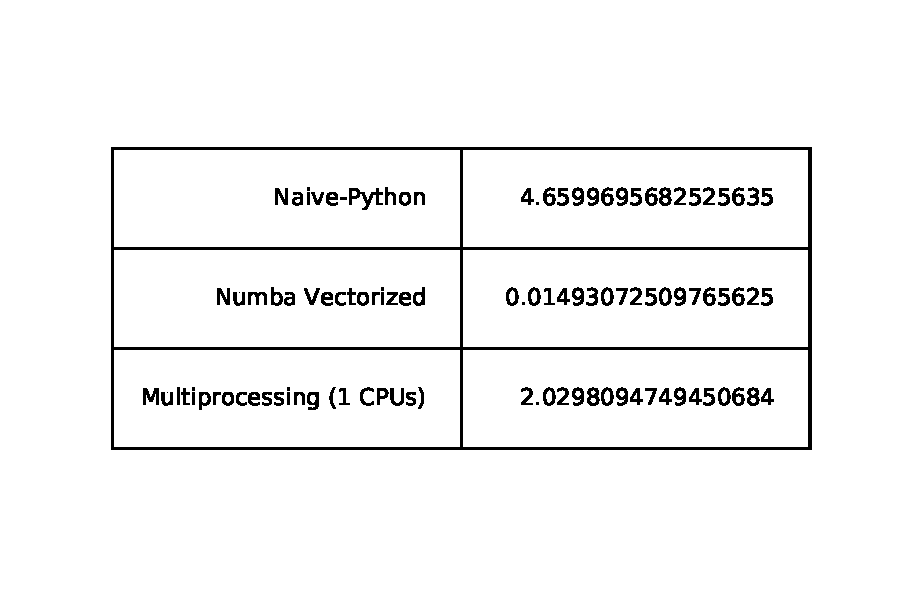
\includegraphics{ExecutionTime.pdf}
    \caption[scale=0.5]{Execution Time}
    \label{fig:exec}
\end{figure}


\subsection{Simulation Data}
The simulation data or the mandelset values generated for each implementation methods are exported as \textit{csv} files in the output folder. 

\section{Software Design}
The software design considerations are described in the following subsections.

\subsection{Design Considerations}
The script is designed to accept input parameters and assumptions from the main method. The input parameters are initialized based on the problem specification provided in the assignment. The values for the threshold, lower bounds, upper bounds are initialized and the values for the number of iterations,  $p_{r_e}$ (height) and $p_{i_m}$ (width) can be provided as per the requirement and system resources.

The main method calls the implementation versions sequentially and records the execution time. The methods for the creation of plots and the tabulation are called after the mandelset computation. The plots, simulation data and execution time are stored in the output directory. The sub-folders are named based on the timestamp of execution.    

\subsection{Optimization Considerations}
The first optimization consideration is to break down the calculation of the mandelset values using the simplified equations specified above. 


\subsection{Algorithm}

\begin{algorithm}[H]
  \caption{Mandelbrot-Set Computation}

  \footnotesize
  \DontPrintSemicolon

  \SetKwInOut{Input}{input}\SetKwInOut{Output}{output}
  \Input{\var{threshold}, \var{Pre}, \var{Pim}, \var{iterations}, \var{Rc(xmin,mmax)}, \var{Ic(ymin,ymax)} \tcc*[f] {specification}}
  \Output{Mandelset \tcc*[f] {Mandelbrot set}}

  \Begin{
    \nl \proc{mandel\_set\_naive}{\var{xmin},\var{xmax},\var{ymin},\var{xmax},\var{Pre},\var{Pim},\var{iter}\var{threshold}}\;
    \nl $\var{r} = \proc{linspace}{\var{xmin},\var{xmax}, \var{Pre}} $ \;
    \nl $\var{i} = \proc{linspace}{\var{ymin},\var{ymax}, \var{Pim}} $\;
    \nl \textbf{/*{Generate the array with the points bounds}*/} \;
    \nl $\var{n} = \var{n[with range Pre-Pim]} $\; 
    \nl \ForEach{x in range Pre}{
        \nl \ForEach{y in range Pim}{
            \nl $\var{n[y][x]} = \proc{mandel\_naive}{\var{complex(r[x], i[y]), \var{iteration}, \var{threshold}}} $
        
    
    \nl $\var{return n}$\;}
    \nl \var{end mandel\_set\_naive()}\;  }
    
    \nl \;
    \nl \proc{mandel\_naive}{\var{c},\var{iteration},\var{threshold}}\;
    \nl $\var{z} = \var{c}$\; 
    \nl \ForEach{n in range maxiter}{
        \If {abs(z) is greater than 2}{
            \Return n
        }
        \nl $z = z*z + c $
    }\nl \Return n\;
    \nl $\var{end}$
      }
    
\end{algorithm}

\section{Test Plan}
The test can be performed with the \textit{mandeltest.py} script. The script tests if the difference of the computed mandelset values is zero. The test for the naive and the numba versions are asserted with \textit{np.testing.assert\_allclose(x,y)}. 


\section{Profiling and Benchmarking}

\begin{align}
    \begin{array}{c | c | c}
         Method  & Execution Time (secs) & Speedup(\%) \\ 
         \hline % horizontal line
         Naive-Numpy   & 4.23 & - \\
         Numba      & 0.57 &  86  \\
         Numba - Vectorized & 0.015 & 99.6 \\
         Multiprocessing(1 CPU) & 1.83 & 56.7 \\
    \end{array}
\end{align}


\begin{figure}[h!]
    \centering
    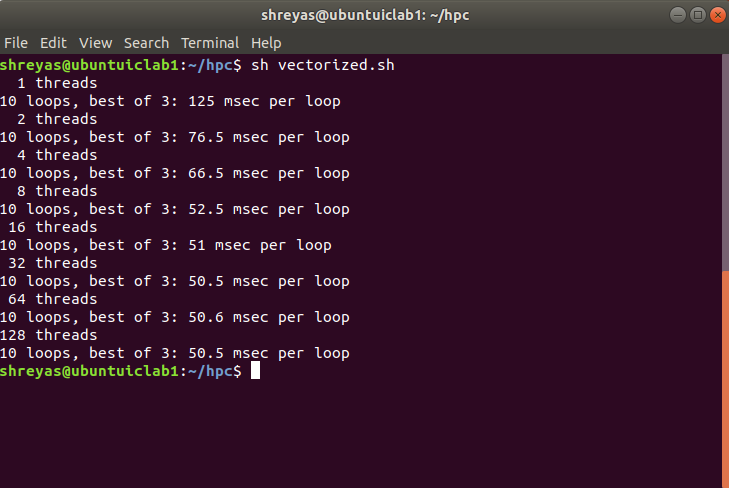
\includegraphics[scale=0.4]{threads_vectorized.png}
    \caption{Numba Vectorized computation time by threads}
    \label{fig:numba_vec}
\end{figure}

\begin{table}[h!]
    \centering
    \begin{align}
    \begin{array}{c | c | c}
         Threads  & Computation Time(msec) & Speedup \\ 
         \hline % horizontal line
         1   & 125 & - \\
         2   & 76.5 &  38.8\%  \\
         4   & 66.5 & 46.8\% \\
         8   & 52.5 & 58\% \\
         16   & 51 & 59.2\% \\
         32   & 50.5 & 59.6\% \\
    \end{array}
\end{align}
    \caption{Computation Time and Speedup - Numba Vectorized}
    \label{tab:my_label}
\end{table}



\begin{figure}
    \centering
    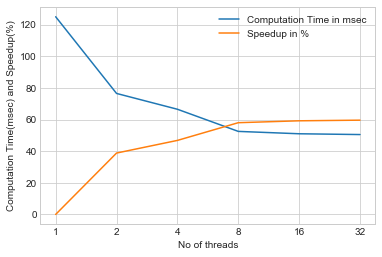
\includegraphics{speedup_plot.png}
    \caption{Computation Time and Speedup Plot for Numba Vectorized Threads}
    \label{fig:my_label}
\end{figure}

\end{document}
